% !TeX encoding = UTF-8
% !TeX program = xelatex
% !TeX spellcheck = en_US

\documentclass[degree=master,fontset=windows]{thuthesis}
  % 学位 degree:
  %   doctor | master | bachelor | postdoc
  % 学位类型 degree-type:
  %   academic(默认)| professional


% 论文基本配置,加载宏包等全局配置
% !TeX root = ../main.tex

% 论文基本信息配置

\thusetup{
  %******************************
  % 注意:
  %   1. 配置里面不要出现空行
  %   2. 不需要的配置信息可以删除
  %******************************
  %
  % 标题
  %   可使用“\\”命令手动控制换行
  %
  title  = {清华大学学位论文 \LaTeX{} 模板\\使用示例文档 v\version},
  title* = {An Introduction to \LaTeX{} Thesis Template of Tsinghua
            University v\version},
  %
  % 学位
  %   1. 学术型
  %      - 中文
  %        需注明所属的学科门类,例如:
  %        哲学、经济学、法学、教育学、文学、历史学、理学、工学、农学、医学、
  %        军事学、管理学、艺术学
  %      - 英文
  %        博士:Doctor of Philosophy
  %        硕士:
  %          哲学、文学、历史学、法学、教育学、艺术学门类,公共管理学科
  %          填写“Master of Arts“,其它填写“Master of Science”
  %   2. 专业型
  %      直接填写专业学位的名称,例如:
  %      教育博士、工程硕士等
  %      Doctor of Education, Master of Engineering
  %   3. 本科生不需要填写
  %
  degree-name  = {工学硕士},
  degree-name* = {Master of Science},
  %
  % 培养单位
  %   填写所属院系的全名
  %
  department = {计算机科学与技术系},
  %
  % 学科
  %   1. 学术型学位
  %      获得一级学科授权的学科填写一级学科名称,其他填写二级学科名称
  %   2. 工程硕士
  %      工程领域名称
  %   3. 其他专业型学位
  %      不填写此项
  %   4. 本科生不需要填写
  %
  discipline  = {计算机科学与技术},
  discipline* = {Computer Science and Technology},
  %
  % 姓名
  %
  author  = {薛瑞尼},
  author* = {Xue Ruini},
  %
  % 指导教师
  %   中文姓名和职称之间以英文逗号“,”分开,下同
  %
  supervisor  = {郑纬民教授},
  supervisor* = {Professor Zheng Weimin},
  %
  % 副指导教师
  %
  % associate-supervisor  = {陈文光教授},
  % associate-supervisor* = {Professor Chen Wenguang},
  %
  % 联合指导教师
  %
  % joint-supervisor  = {某某某教授},
  % joint-supervisor* = {Professor Mou Moumou},
  %
  % 日期
  %   使用 ISO 格式;默认为当前时间
  %
  % date = {2019-07-07},
  %
  % 密级和年限
  %   秘密, 机密, 绝密
  %
  % secret-level = {秘密},
  % secret-year  = {10},
  %
  % 博士后专有部分
  %
  % clc                = {分类号},
  % udc                = {UDC},
  % id                 = {编号},
  % discipline-level-1 = {计算机科学与技术},  % 流动站(一级学科)名称
  % discipline-level-2 = {系统结构},          % 专业(二级学科)名称
  % start-date         = {2011-07-01},        % 研究工作起始时间
}

%% Put any packages you would like to use here

% 表格中支持跨行
\usepackage{multirow}

% 跨页表格
\usepackage{longtable}

% 固定宽度的表格
\usepackage{tabularx}

% 表格中的反斜线
\usepackage{diagbox}

% 确定浮动对象的位置,可以使用 H,强制将浮动对象放到这里(可能效果很差)
\usepackage{float}

% 浮动图形控制宏包。
% 允许上一个 section 的浮动图形出现在下一个 section 的开始部分
% 该宏包提供处理浮动对象的 \FloatBarrier 命令,使所有未处
% 理的浮动图形立即被处理。这三个宏包仅供参考,未必使用:
% \usepackage[below]{placeins}
% \usepackage{floatflt} % 图文混排用宏包
% \usepackage{rotating} % 图形和表格的控制旋转

% 定理类环境宏包
\usepackage[amsmath,thmmarks,hyperref]{ntheorem}

% 给自定义的宏后面自动加空白
% \usepackage{xspace}

% 借用 ltxdoc 里面的几个命令。
\def\cmd#1{\cs{\expandafter\cmd@to@cs\string#1}}
\def\cmd@to@cs#1#2{\char\number`#2\relax}
\DeclareRobustCommand\cs[1]{\texttt{\char`\\#1}}

\newcommand*{\meta}[1]{{%
  \ensuremath{\langle}\rmfamily\itshape#1\/\ensuremath{\rangle}}}
\providecommand\marg[1]{%
  {\ttfamily\char`\{}\meta{#1}{\ttfamily\char`\}}}
\providecommand\oarg[1]{%
  {\ttfamily[}\meta{#1}{\ttfamily]}}
\providecommand\parg[1]{%
  {\ttfamily(}\meta{#1}{\ttfamily)}}
\providecommand\pkg[1]{{\sffamily#1}}

% 定义所有的图片文件在 figures 子目录下
\graphicspath{{figures/}}

% 数学命令
% Adapted for use with thuthesis.
% Original code is at https://github.com/goodfeli/dlbook_notation/blob/master/math_commands.tex

%%%%% NEW MATH DEFINITIONS %%%%%

\newcommand\ceil[1]{\lceil #1 \rceil}
\newcommand\floor[1]{\lfloor #1 \rfloor}


% Vectors
% \newcommand\Vector[1]{\symbf{#1}}

\newcommand\0{{\Vector{0}}}
\newcommand\vzero{{\Vector{0}}}
\newcommand\1{{\Vector{1}}}
\newcommand\vone{{\Vector{1}}}

\newcommand\va{{\Vector{a}}}
\newcommand\vb{{\Vector{b}}}
\newcommand\vc{{\Vector{c}}}
\newcommand\vd{{\Vector{d}}}
\newcommand\ve{{\Vector{e}}}
\newcommand\vf{{\Vector{f}}}
\newcommand\vg{{\Vector{g}}}
\newcommand\vh{{\Vector{h}}}
\newcommand\vi{{\Vector{i}}}
\newcommand\vj{{\Vector{j}}}
\newcommand\vk{{\Vector{k}}}
\newcommand\vl{{\Vector{l}}}
\newcommand\vm{{\Vector{m}}}
\newcommand\vn{{\Vector{n}}}
\newcommand\vo{{\Vector{o}}}
\newcommand\vp{{\Vector{p}}}
\newcommand\vq{{\Vector{q}}}
\newcommand\vr{{\Vector{r}}}
\newcommand\vs{{\Vector{s}}}
\newcommand\vt{{\Vector{t}}}
\newcommand\vu{{\Vector{u}}}
\newcommand\vv{{\Vector{v}}}
\newcommand\vw{{\Vector{w}}}
\newcommand\vx{{\Vector{x}}}
\newcommand\vy{{\Vector{y}}}
\newcommand\vz{{\Vector{z}}}

\newcommand\valpha{{\Vector{\alpha}}}
\newcommand\vbeta{{\Vector{\beta}}}
\newcommand\vgamma{{\Vector{\gamma}}}
\newcommand\vdelta{{\Vector{\delta}}}
\newcommand\vepsilon{{\Vector{\epsilon}}}
\newcommand\vtheta{{\Vector{\theta}}}
\newcommand\viota{{\Vector{\iota}}}
\newcommand\vkappa{{\Vector{\kappa}}}
\newcommand\vlambda{{\Vector{\lambda}}}
\newcommand\vmu{{\Vector{\mu}}}
\newcommand\vnu{{\Vector{\nu}}}
\newcommand\vxi{{\Vector{\xi}}}
\newcommand\vpi{{\Vector{\pi}}}
\newcommand\vrho{{\Vector{\rho}}}
\newcommand\vsigma{{\Vector{\sigma}}}
\newcommand\vtau{{\Vector{\tau}}}
\newcommand\vupsilon{{\Vector{\upsilon}}}
\newcommand\vphi{{\Vector{\phi}}}
\newcommand\vchi{{\Vector{\chi}}}
\newcommand\vpsi{{\Vector{\psi}}}
\newcommand\vomega{{\Vector{\omega}}}


% Matrix
\newcommand\MATRIX[1]{\symbf{#1}}

\newcommand\mA{{\MATRIX{A}}}
\newcommand\mB{{\MATRIX{B}}}
\newcommand\mC{{\MATRIX{C}}}
\newcommand\mD{{\MATRIX{D}}}
\newcommand\mE{{\MATRIX{E}}}
\newcommand\mF{{\MATRIX{F}}}
\newcommand\mG{{\MATRIX{G}}}
\newcommand\mH{{\MATRIX{H}}}
\newcommand\mI{{\MATRIX{I}}}
\newcommand\mJ{{\MATRIX{J}}}
\newcommand\mK{{\MATRIX{K}}}
\newcommand\mL{{\MATRIX{L}}}
\newcommand\mM{{\MATRIX{M}}}
\newcommand\mN{{\MATRIX{N}}}
\newcommand\mO{{\MATRIX{O}}}
\newcommand\mP{{\MATRIX{P}}}
\newcommand\mQ{{\MATRIX{Q}}}
\newcommand\mR{{\MATRIX{R}}}
\newcommand\mS{{\MATRIX{S}}}
\newcommand\mT{{\MATRIX{T}}}
\newcommand\mU{{\MATRIX{U}}}
\newcommand\mV{{\MATRIX{V}}}
\newcommand\mW{{\MATRIX{W}}}
\newcommand\mX{{\MATRIX{X}}}
\newcommand\mY{{\MATRIX{Y}}}
\newcommand\mZ{{\MATRIX{Z}}}

\newcommand\mGamma{{\MATRIX{\Gamma}}}
\newcommand\mDelta{{\MATRIX{\Delta}}}
\newcommand\mTheta{{\MATRIX{\Theta}}}
\newcommand\mLambda{{\MATRIX{\Lambda}}}
\newcommand\mXi{{\MATRIX{\Xi}}}
\newcommand\mPi{{\MATRIX{\Pi}}}
\newcommand\mSigma{{\MATRIX{\Sigma}}}
\newcommand\mUpsilon{{\MATRIX{\Upsilon}}}
\newcommand\mPhi{{\MATRIX{\Phi}}}
\newcommand\mPsi{{\MATRIX{\Psi}}}
\newcommand\mOmega{{\MATRIX{\Omega}}}


% Tensor
\newcommand\tens[1]{\symbfsf{#1}}
\newcommand\tA{{\tens{A}}}
\newcommand\tB{{\tens{B}}}
\newcommand\tC{{\tens{C}}}
\newcommand\tD{{\tens{D}}}
\newcommand\tE{{\tens{E}}}
\newcommand\tF{{\tens{F}}}
\newcommand\tG{{\tens{G}}}
\newcommand\tH{{\tens{H}}}
\newcommand\tI{{\tens{I}}}
\newcommand\tJ{{\tens{J}}}
\newcommand\tK{{\tens{K}}}
\newcommand\tL{{\tens{L}}}
\newcommand\tM{{\tens{M}}}
\newcommand\tN{{\tens{N}}}
\newcommand\tO{{\tens{O}}}
\newcommand\tP{{\tens{P}}}
\newcommand\tQ{{\tens{Q}}}
\newcommand\tR{{\tens{R}}}
\newcommand\tS{{\tens{S}}}
\newcommand\tT{{\tens{T}}}
\newcommand\tU{{\tens{U}}}
\newcommand\tV{{\tens{V}}}
\newcommand\tW{{\tens{W}}}
\newcommand\tX{{\tens{X}}}
\newcommand\tY{{\tens{Y}}}
\newcommand\tZ{{\tens{Z}}}


% Graph
\newcommand\gA{{\mathcal{A}}}
\newcommand\gB{{\mathcal{B}}}
\newcommand\gC{{\mathcal{C}}}
\newcommand\gD{{\mathcal{D}}}
\newcommand\gE{{\mathcal{E}}}
\newcommand\gF{{\mathcal{F}}}
\newcommand\gG{{\mathcal{G}}}
\newcommand\gH{{\mathcal{H}}}
\newcommand\gI{{\mathcal{I}}}
\newcommand\gJ{{\mathcal{J}}}
\newcommand\gK{{\mathcal{K}}}
\newcommand\gL{{\mathcal{L}}}
\newcommand\gM{{\mathcal{M}}}
\newcommand\gN{{\mathcal{N}}}
\newcommand\gO{{\mathcal{O}}}
\newcommand\gP{{\mathcal{P}}}
\newcommand\gQ{{\mathcal{Q}}}
\newcommand\gR{{\mathcal{R}}}
\newcommand\gS{{\mathcal{S}}}
\newcommand\gT{{\mathcal{T}}}
\newcommand\gU{{\mathcal{U}}}
\newcommand\gV{{\mathcal{V}}}
\newcommand\gW{{\mathcal{W}}}
\newcommand\gX{{\mathcal{X}}}
\newcommand\gY{{\mathcal{Y}}}
\newcommand\gZ{{\mathcal{Z}}}


% Sets
\newcommand\sA{{\mathbb{A}}}
\newcommand\sB{{\mathbb{B}}}
\newcommand\sC{{\mathbb{C}}}
\newcommand\sD{{\mathbb{D}}}
% Don't use a set called E, because this would be the same as our symbol
% for expectation.
\newcommand\sF{{\mathbb{F}}}
\newcommand\sG{{\mathbb{G}}}
\newcommand\sH{{\mathbb{H}}}
\newcommand\sI{{\mathbb{I}}}
\newcommand\sJ{{\mathbb{J}}}
\newcommand\sK{{\mathbb{K}}}
\newcommand\sL{{\mathbb{L}}}
\newcommand\sM{{\mathbb{M}}}
\newcommand\sN{{\mathbb{N}}}
\newcommand\sO{{\mathbb{O}}}
\newcommand\sP{{\mathbb{P}}}
\newcommand\sQ{{\mathbb{Q}}}
\newcommand\sR{{\mathbb{R}}}
\newcommand\sS{{\mathbb{S}}}
\newcommand\sT{{\mathbb{T}}}
\newcommand\sU{{\mathbb{U}}}
\newcommand\sV{{\mathbb{V}}}
\newcommand\sW{{\mathbb{W}}}
\newcommand\sX{{\mathbb{X}}}
\newcommand\sY{{\mathbb{Y}}}
\newcommand\sZ{{\mathbb{Z}}}


% Random variables
\newcommand\RandomVariable[1]{\symit{#1}}

\newcommand\rA{{\RandomVariable{A}}}
\newcommand\rB{{\RandomVariable{B}}}
\newcommand\rC{{\RandomVariable{C}}}
\newcommand\rD{{\RandomVariable{D}}}
\newcommand\rE{{\RandomVariable{E}}}
\newcommand\rF{{\RandomVariable{F}}}
\newcommand\rG{{\RandomVariable{G}}}
\newcommand\rH{{\RandomVariable{H}}}
\newcommand\rI{{\RandomVariable{I}}}
\newcommand\rJ{{\RandomVariable{J}}}
\newcommand\rK{{\RandomVariable{K}}}
\newcommand\rL{{\RandomVariable{L}}}
\newcommand\rM{{\RandomVariable{M}}}
\newcommand\rN{{\RandomVariable{N}}}
\newcommand\rO{{\RandomVariable{O}}}
\newcommand\rP{{\RandomVariable{P}}}
\newcommand\rQ{{\RandomVariable{Q}}}
\newcommand\rR{{\RandomVariable{R}}}
\newcommand\rS{{\RandomVariable{S}}}
\newcommand\rT{{\RandomVariable{T}}}
\newcommand\rU{{\RandomVariable{U}}}
\newcommand\rV{{\RandomVariable{V}}}
\newcommand\rW{{\RandomVariable{W}}}
\newcommand\rX{{\RandomVariable{X}}}
\newcommand\rY{{\RandomVariable{Y}}}
\newcommand\rZ{{\RandomVariable{Z}}}

% Random vectors
\newcommand\RandomVector[1]{\symbf{#1}}

\newcommand\rvA{{\RandomVector{A}}}
\newcommand\rvB{{\RandomVector{B}}}
\newcommand\rvC{{\RandomVector{C}}}
\newcommand\rvD{{\RandomVector{D}}}
\newcommand\rvE{{\RandomVector{E}}}
\newcommand\rvF{{\RandomVector{F}}}
\newcommand\rvG{{\RandomVector{G}}}
\newcommand\rvH{{\RandomVector{H}}}
\newcommand\rvI{{\RandomVector{I}}}
\newcommand\rvJ{{\RandomVector{J}}}
\newcommand\rvK{{\RandomVector{K}}}
\newcommand\rvL{{\RandomVector{L}}}
\newcommand\rvM{{\RandomVector{M}}}
\newcommand\rvN{{\RandomVector{N}}}
\newcommand\rvO{{\RandomVector{O}}}
\newcommand\rvP{{\RandomVector{P}}}
\newcommand\rvQ{{\RandomVector{Q}}}
\newcommand\rvR{{\RandomVector{R}}}
\newcommand\rvS{{\RandomVector{S}}}
\newcommand\rvT{{\RandomVector{T}}}
\newcommand\rvU{{\RandomVector{U}}}
\newcommand\rvV{{\RandomVector{V}}}
\newcommand\rvW{{\RandomVector{W}}}
\newcommand\rvX{{\RandomVector{X}}}
\newcommand\rvY{{\RandomVector{Y}}}
\newcommand\rvZ{{\RandomVector{Z}}}

\newcommand\laplace{\mathrm{Laplace}} % Laplace distribution

\newcommand\E{\mathbb{E}}
\newcommand\Ls{\mathcal{L}}
\newcommand\R{\mathbb{R}}
\newcommand\emp{\tilde{p}}
\newcommand\lr{\alpha}
\newcommand\reg{\lambda}
\newcommand\rect{\mathrm{rectifier}}
\newcommand\softmax{\mathrm{softmax}}
\newcommand\sigmoid{\sigma}
\newcommand\softplus{\zeta}
\newcommand\KL{D_{\mathrm{KL}}}
\newcommand\Var{\mathrm{Var}}
\newcommand\standarderror{\mathrm{SE}}
\newcommand\Cov{\mathrm{Cov}}
% Wolfram Mathworld says $L^2$ is for function spaces and $\ell^2$ is for vectors
% But then they seem to use $L^2$ for vectors throughout the site, and so does
% wikipedia.
\newcommand\normlzero{L^0}
\newcommand\normlone{L^1}
\newcommand\normltwo{L^2}
\newcommand\normlp{L^p}
\newcommand\normmax{L^\infty}

\DeclareMathOperator*{\argmax}{arg\,max}
\DeclareMathOperator*{\argmin}{arg\,min}

\DeclareMathOperator{\sign}{sign}
\DeclareMathOperator{\Tr}{Tr}
\let\ab\allowbreak


% 定义自己常用的东西
% \def\myname{薛瑞尼}

% hyperref 宏包在最后调用
\usepackage{hyperref}



\begin{document}

% 封面
\maketitle

% 使用授权的说明
\copyrightpage

\frontmatter
% !TeX root = ../main.tex

% 中英文摘要和关键字

\begin{abstract}
  可用性是分布式文件系统的重要属性之一。近年来,持久性内存(NVM)技术出现并高速发展,给这一领域带来了新的机遇。通过合理地利用 NVM 高速、字节粒度访问的特性,系统能够以更低的开销、更高的速度提供高可用的文件存储服务。

  本文提出一种面向 NVM 存储的分布式文件系统。该系统使用纠删码提供可用性保障,其性能不低于使用备份策略的传统分布式文件系统,并且在相同容错条件下显著节省所需的存储空间。测试显示。

  % 关键词用“英文逗号”分隔
  \thusetup{
    keywords = {NVM, RDMA, 分布式文件系统, 可用性},
  }
\end{abstract}

\begin{abstract*}
  Availability is a key feature of distributed file systems. In recent years, the advent and rapid development of non-volatile memory (NVM) technology brings new chances to this field. By leveraging the high-performance and byte-addressable features of NVMs, the system can provide file storage service with lower cost, higher speed, and together with high availability.

  In this paper, we present a new distributed file system for NVM-based storage, which uses erasure codes to guarantee its availability. It performs no worse than traditional systems using replication as their availability strategy, while using far less storage with the same fault-tolerance ability. Evaluations show that. 

  \thusetup{
    keywords* = {NVM, RDMA, distributed file system, availability},
  }
\end{abstract*}


% 目录
\tableofcontents

% 符号对照表
% !TeX root = ../main.tex

\begin{denotation}[3cm]
\item[HDD]  机械硬盘(Hard Disk Drive)
\item[SSD]  固态硬盘(Solid State Drive)
\item[DFS]  分布式文件系统(Distributed File System)
\item[NVM]  持久性内存(Non-volatile Memory)
\item[RDMA] 远程直接内存访问(Remote Direct Memory Access)
\end{denotation}



% 正文部分
\mainmatter
% !TeX root = ../main.tex

\chapter{引言}
\label{cha:intro}

% 本课题问题的提出、意义及实用价值;已有研究情况的概述;本课题所要解决的问题等。

\section{研究背景}
\label{sec:ch1_background}

文件是用于数据处理的最基本的抽象之一。日益增长的互联网规模正带来日益增长的文件存储需求;单机文件系统早已无法应对如此巨大的数据量,分布式文件系统(Distributed File System,DFS)应运而生。相比于单机系统,DFS 具有高性能、高并发度和良好的可扩展性,已经成为近年来的热点研究方向。

DFS 通常包含三个最主要的部分:存储、计算和网络通信,系统的性能由这三者共同决定。由于三者各自的性能互不相同,平衡三者的性能从而优化整个系统成为了近年来分布式文件系统方向研究的主流方向。另外,组成 DFS的单机彼此之间在物理上分离。在共同提供单机所无法比拟的数据处理能力的同时,它们也可能各自独立地发生故障,从而使得整个系统发生故障的概率大大提高。因此,DFS 通常必须引入额外的存储、计算和网络通信,从而提供可用性保障,即是说,系统在某些节点故障时应该仍然能正常工作。如何在三者性能损失和系统可用性之间权衡,是 DFS 设计中另一个必须考虑的问题。

传统 DFS 通常使用机械式磁盘(Hard Disk Drive,HDD)或固态硬盘(Solid State Drive,SSD)作为其持久性存储介质。它们的优点是容量较大:如 Seagate 公司已经生产出容量达 16TB 的商用 HDD,SanDisk 公司也已制造出容量达 8TB 的 SSD 原型;缺点则是访问延迟也较大:HDD 的随机访问由于寻道、磁盘旋转等延迟的存在通常需要花费数个毫秒,SSD 的平均访问延迟也通常达到数百微秒。这种访问特性使得存储部分成为整个 DFS 的瓶颈。基于传统存储介质的 DFS 的典型例子如 Ceph\cite{ceph2006}、HDFS\cite{hadoop2010} 和 Gluster\cite{gluster2013}。它们通常针对系统中性能最低的存储介质读写进行优化,同时占用 CPU 进行大量运算(例如,Ceph 定期执行的 compaction 操作会带来巨大 CPU 负载)。为了保证可用性,这些文件系统通常会存储数据的若干个备份,防止单节点故障导致数据无法访问。

近年来,持久性内存(Non-volatile Memory,NVM)技术的迅速发展打破了这种设计范式。与传统的持久性存储介质相比,NVM 同样具有断电不丢失数据的优点;同时,它支持字节粒度访问,读写延迟低三到四个数量级。例如,Intel 公司 Optane\textsuperscript{\texttrademark} SSD 产品的 4KB 随机读写延迟约为 $\SI{214}{\us}$\cite{optanessd},而其 Optane\textsuperscript{\texttrademark} DC NVM 产品的 4KB 随机读延迟约为 $\SI{0.3}{\us}$,随机写速度更是低至 0.06 $\sim \SI{0.09}{\us}$\cite{yangnvm2020}。在这种情况下,传统 DFS 对存储介质读写的优化就显得无足轻重;而同时,CPU 的计算资源和网络带宽反而成为了新的瓶颈。因此,基于大容量、低速存储介质的传统 DFS 在 NVM 的这些新特性面前不再适用。发展适合 NVM 特性的新型高可用 DFS势在必行。

基于 NVM 的分布式文件系统的一个核心问题是其存储成本。由于 HDD、SSD 技术都早已成熟,单位容量价格十分低廉,传统 DFS 可以存储数据的多个副本,而不必担心因此产生过多的额外花销。NVM 单位容量的价格则较为昂贵,如果直接应用既有的可用性策略,则势必产生巨大的存储成本。如何在保证 DFS 高效率的同时尽可能减少存储开销,仍然是一个开放问题,既往研究几乎没有涉及。

纠删码是一种较为新型的数据容错策略,它在电子通信领域已经得到广泛应用:只需额外传输很少的额外数据,就能提供较高的容错能力。因此,在节省存储开销方面,纠删码有着巨大的潜力。在文件系统领域,也已有许多工作使用了纠删码,但它在基于 NVM 的分布式系统中表现如何尚未有定论。因此,本课题的目标是在 NVM+RDMA 环境下实现纠删码,并以此为文件系统中的数据提供可用性保障,最后测试其性能表现。

\section{研究现状}
\label{sec:ch1_relworks}

本小节从基于 NVM 的文件系统和纠删码两方面介绍学术界目前的研究情况。

\subsection{基于 NVM 的文件系统}
\label{subsec:ch1_nvm_relworks}

NVM 技术在近两三年发展迅速。早期的一些工作提出使用 NVM 代替 HDD、SSD 等低速存储介质,从而提高单机文件系统的性能。已有的成果如加州大学圣迭戈分校提出的 NOVA\cite{nova2016} 和它的改进 NOVA-Fortis\cite{novafortis2017}。NOVA 利用了 NVM 的字节粒度访问的特性,将文件系统日志存储在 NVM 中,减少了日志持久化带来的开销。NOVA-Fortis 在此基础上还提供了数据完整性的保障。

另外,也已有多项研究开始使用 NVM 作为 DFS 中的持久性存储介质。由于数据存储的延迟已经极大地降低,传统的基于 TCP/IP 网络协议栈的网络通信成为了新的性能瓶颈。新兴的远程内存直接访问(Remote Direct Memory Access,RDMA)技术支持用户态直接访问远端节点的内存,减少了大量的数据复制,很大程度上缓解了这一问题。综合利用 NVM 和 RDMA 技术的已有成果如清华大学提出的 Octopus\cite{octopus2017}、加州大学圣迭戈分校提出的 Orion\cite{orion2019} 和华盛顿大学提出的 Assise\cite{assise2019}。它们从不同方面入手优化文件系统的性能。例如,Octopus 改进了分布式事务协议来降低网络请求的开销;Orion 借鉴了 NOVA,通过一个高效的元数据服务器降低维持一致性的开销;Assise 则实现了完善的缓存机制,通过多级备份实现快速的错误恢复。

然而,上述这些研究使用的仍是备份策略,忽视了当前高成本 NVM 带来的节省存储空间的需求。尚未有已发表的工作研究如何以较低的 NVM 空间开销保证系统的高可用性。

\subsection{基于纠删码的文件系统可用性策略}
\label{subsec:ch1_ec_relworks}

纠删码早在 1950 年代就出现在通信领域,其代表是 Hamming 码,可以识别和纠正通信中的任意单比特错误。在存储领域,纠删码已经被应用于前沿研究和工程实际中。

前沿研究方面,上海交通大学提出的 Cocytus\cite{cocytus2016} 在一个内存键值存储引擎中应用了纠删码策略;乔治·梅森大学提出的 InfiniCache\cite{infinicache2020} 构建了一个大规模分布式数据缓存系统,同样应用了纠删码,以提供数据可用性保障、提升效率和降低成本;密歇根大学提出的 Hydra\cite{hydra2019} 则构建了一个使用纠删码策略的分布式内存分配器。这些研究表明了在高性能系统中使用纠删码的可行性和有效性。

工程实际方面,微软公司早在 2012 年就在其 Windows Azure 云存储系统中部署了一个低开销的纠删码策略\cite{azure2012},用于应对 Azure 存储服务器频繁的下线更新,使系统始终保持可用。Facebook 公司也使用了一个称为 f4 的纠删码存储系统\cite{facebook2014},用于以较低的空间开销存储 Facebook 上大量的图片和流媒体文件。这些纠删码的应用实例表明了纠删码用于文件系统时带来的明显优势。

然而,这些系统或者不是标准的分布式文件系统,不能代表纠删码在文件系统中的性能表现;或者基于传统块设备设计,并且已经有一定的历史,不能适应基于 NVM+RDMA 的最新存储环境。尚未有已发表的工作研究如何在高性能存储和网络环境下应用纠删码策略。

\section{本课题解决的问题}
\label{sec:ch1_thiswork}

既往研究已经揭示了纠删码作为分布式存储系统的可用性保障的潜力。但是,尚未有研究在 NVM+RDMA 环境下构建一个使用纠删码的 DFS,通过实证的方式检验纠删码的可行性和有效性。本课题首先作出了填补这一空白的尝试。具体而言,本课题解决的问题是:证明在 NVM 作为存储介质、RDMA 提供高速高带宽网络的环境下,纠删码是一种合适的可用性方案,其能在节省存储空间的同时,又保证较好的性能。

为了实现上述研究目标,本课题采取了以下的研究方案:首先,设计并实现一个基于 NVM 和 RDMA 的新型分布式文件系统。该系统采用模块化的设计方式,针对 NVM+RDMA 环境对现有的纠删码策略进行优化、移植。完成系统的设计后,从理论上证明,相较于传统数据备份策略,使用纠删码能带来更低的存储开销。完成系统的实现后,对该系统开展综合的测试,与传统数据备份策略对比,证明纠删码能提供与之相当的可用性保障,同时也能提供与之相当或更优的性能。

% !TeX root = ../main.tex

\chapter{图表公式例子}
\label{cha:chapter02}

\section{其它例子}
\label{sec:other}

在第~\ref{cha:intro} 章中我们学习了贝叶斯公式~(\ref{equ:chap1:bayes}),这里我们复
习一下:
\begin{equation}
\label{equ:chap2:bayes}
p(y|\vx) = \frac{p(\vx,y)}{p(\vx)}=
\frac{p(\vx|y)p(y)}{p(\vx)}
\end{equation}

\subsection{绘图}
\label{sec:draw}

本模板不再预先装载任何绘图包(如 \pkg{pstricks,pgf} 等),完全由用户来决定。
个人觉得 \pkg{pgf} 不错,不依赖于 Postscript。此外还有很多针对 \LaTeX{} 的
 GUI 作图工具,如 XFig(jFig), WinFig, Tpx, Ipe, Dia, Inkscape, LaTeXPiX,
jPicEdt, jaxdraw 等等。

\subsection{插图}
\label{sec:graphs}

强烈推荐《\LaTeXe{} 插图指南》!关于子图形的使用细节请参看 \pkg{subcaption} 宏包的说明文档。

\subsubsection{一个图形}
\label{sec:onefig}
一般图形都是处在浮动环境中。之所以称为浮动是指最终排版效果图形的位置不一定与源文
件中的位置对应\footnote{This is not a bug, but a feature of \LaTeX!},这也是刚使
用 \LaTeX{} 同学可能遇到的问题。如果要强制固定浮动图形的位置,请使用 \pkg{float} 宏包,
它提供了 \texttt{[H]} 参数,比如图~\ref{fig:xfig1}。
\begin{figure}[H] % use float package if you want it here
  \centering
  
\includegraphics{thu-whole-logo.pdf}
  \caption{利用 Xfig 制图}
  \label{fig:xfig1}
\end{figure}

大学之道,在明明德,在亲民,在止于至善。知止而后有定;定而后能静;静而后能安;安
而后能虑;虑而后能得。物有本末,事有终始。知所先后,则近道矣。古之欲明明德于天
下者,先治其国;欲治其国者,先齐其家;欲齐其家者,先修其身;欲修其身者,先正其心;
欲正其心者,先诚其意;欲诚其意者,先致其知;致知在格物。物格而后知至;知至而后
意诚;意诚而后心正;心正而后身 修;身修而后家齐;家齐而后国治;国治而后天下
平。自天子以至于庶人,壹是皆以修身为本。其本乱而未治者 否矣。其所厚者薄,而其所
薄者厚,未之有也!

\hfill —— 《大学》


\subsubsection{多个图形}
\label{sec:multifig}

如果多个图形相互独立,并不共用一个图形计数器,那么
用 \texttt{minipage} 或者\texttt{parbox} 就可以。否则,请参看
图~\ref{fig:big1-subcaptionbox},它包含两个小图,分别是图~\ref{fig:subfig1}和
图~\ref{fig:subfig2}。推荐使用 \cs{subcaptionbox},因为可以像
图~\ref{fig:big1-subcaptionbox} 那样对齐子图的标题,也可以使用 \pkg{subcaption}
宏包的 \cs{subcaption}(放在 minipage中,用法同\cs{caption})或
是 \pkg{subfigure} 、\pkg{subtable}环境,像图~\ref{fig:big1-subfigure},不要再
用 \cs{subfloat}、\cs{subfigure} 和 \cs{subtable}。

\begin{figure}[h]
  \centering%
  \subcaptionbox{第一个小图形\label{fig:subfig1}}[3cm] %标题的长度,超过则会换行,如下一个小图。
    {
\includegraphics[height=3cm]{thu-fig-logo.pdf}}%
  \hspace{4em}%
  \subcaptionbox{第二个小图形,注意这个图略矮些。如果标题很长的话,它会自动换行\label{fig:subfig2}}
      {
\includegraphics[height=2cm]{thu-text-logo.pdf}}
  \caption{包含子图形的大图形(subcaptionbox示例)}
  \label{fig:big1-subcaptionbox}
\end{figure}
\begin{figure}[h]
  \centering%
  \begin{subfigure}{3cm}
    
\includegraphics[height=3cm]{thu-fig-logo.pdf}
    \caption{第一个小图形}
  \end{subfigure}%
  \hspace{4em}%
  \begin{subfigure}{0.5\textwidth}
    
\includegraphics[height=2cm]{thu-text-logo.pdf}
    \caption{第二个小图形,注意这个图略矮些。subfigure中同一行的子图在顶端对齐。}
  \end{subfigure}
  \caption{包含子图形的大图形(subfigure示例)}
  \label{fig:big1-subfigure}
\end{figure}

古之学者必有师。师者,所以传道受业解惑也。人非生而知之者,孰能无惑?惑而不从师,
其为惑也,终不解矣。生乎吾前,其闻道也固先乎吾,吾从而师之;生乎吾後,其闻道也亦
先乎吾,吾从而师之。吾师道也,夫庸知其年之先後生於吾乎!是故无贵无贱无长无少,道
之所存,师之所存也。

嗟乎!师道之不传也久矣,欲人之无惑也难矣。古之圣人,其出人也远矣,犹且从师而问焉;
今之众人,其下圣人也亦远矣,而耻学於师。是故圣益圣,愚益愚。圣人之所以为圣,愚
人之所以为愚,其皆出於此乎?爱其子,择师而教之,於其身也,则耻师焉,惑焉。彼童子
之师,授之书而习其句读者,非吾所谓传其道、解其惑者也。句读之不知,惑之不解,或师
焉,或不焉,小学而大遗,吾未见其明也。巫医、乐师、百工之人不耻相师,  士大夫之族
曰“师”曰“弟子”之云者,则群聚而笑之。问之,则曰:彼与彼年相若也,道相似也,位
卑则足羞,官盛则近谀。呜呼!师道之不复,可知矣。巫医、乐师、百工之人。吾子不齿,
今其智乃反不能及,其可怪也欤!圣人无常师。孔子师郯子、苌子、师襄、老聃。郯子之徒,
其贤不及孔子。孔子曰:“三人行,必有我师。”是故弟子不必不如师,师不必贤於弟子。
闻道有先後,术业有专攻,如是而已。

如果要把编号的两个图形并排,那么小页就非常有用了:
\begin{figure}
\begin{minipage}{0.48\textwidth}
  \centering
  
\includegraphics[height=2cm]{thu-whole-logo.pdf}
  \caption{并排第一个图}
  \label{fig:parallel1}
\end{minipage}\hfill
\begin{minipage}{0.48\textwidth}
  \centering
  
\includegraphics[height=2cm]{thu-whole-logo.pdf}
  \caption{并排第二个图}
  \label{fig:parallel2}
\end{minipage}
\end{figure}

李氏子蟠,年十七,好古文、六艺,经传皆通习之,不拘於时,学於余。余嘉其能行古
道,作师说以贻之。

\hfill —— 韩愈(唐)



% 其它部分
\backmatter

%% 本科生要求的几个索引。
% \listoffigures    % 插图索引
% \listoftables     % 表格索引
% \listofequations  % 公式索引

% 参考文献
\bibliographystyle{thuthesis-numeric}      % 顺序编码制
% \bibliographystyle{thuthesis-author-year}  % 著者-出版年制
% \bibliographystyle{thuthesis-bachelor}     % 本科生参考文献的著录格式
\bibliography{ref/refs}

% 致谢
% !TeX root = ../main.tex

\begin{acknowledgements}
  感谢导师舒继武教授、陆游游助理教授为我的研究全程提供指导和建议。

  感谢吕文豪学长为我提供了 LocoFS 的源代码和使用指导。感谢汪庆学长、朱博弘学长为我提供测试服务器,并且帮助我解决在使用过程中遇到的各种问题。

  感谢 \thuthesis\cite{thuthesis} 提供了功能齐全的模板,极大地方便了本文的撰写工作。
\end{acknowledgements}


% 声明
\statement

% 附录
\appendix
% % !TeX root = ../main.tex

\begin{survey}
\label{cha:survey}

\title{Literature Review of RDMA-Enabled Distributed File Systems on NVM}
\maketitle

High-performance, byte-addressable non-volatile memories (NVMs) developed dramatically and have been the cutting-edge of storage systems in recent years. Prior to its advent, distributed system designers find that the system’s performance is mainly limited by the access latency of the underlying block device. Both hard-disks and solid-state drives (SSDs) are much slower than DRAM, leading to complex, specialized designs for better efficiency \cite{sorion2019}.

However, the appearance of NVM brings us low-cost, high-capacity and byte-addressable fast persistent data storage. Media access latency no longer determines the whole system’s performance, which forces designers to rethink those tradeoffs with networking overhead and CPU involvement \cite{sorion2019}. With remote direct memory access (RDMA), NVM access over the InfiniBand network is also efficient enough, promising a bright future for RDMA-based NVM distributed storage systems \cite{sassise2019}.

Many new file systems are designed to fully exploit the features of NVM and RDMA for better performance. They share the same design principle, that the overheads of kernel/user crossing and network accesses should be reduced to minimal. All these systems must provide data consistency, while they can also have additional features like availability, fault tolerance, and failure recovery. Due to the CAP Theorem, they must make different tradeoffs among these features, resulting in the diversity of these systems. {\em Octopus} \cite{soctopus2017}, {\em Orion} \cite{sorion2019}, and {\em Assise} \cite{sassise2019} are three typical examples of NVM-specialized distributed file systems. Octopus was first published in 2017, and Orion and Assise were both published in 2019.

\section{Octopus}
Octopus exploits the fact that a remote procedure call (RPC) is much more expensive than an RDMA verb. From this fact, Octopus stated that the client should actively fetch data from the server, instead of incurring an RPC request and simply waiting for the server to prepare the data and send it back. We may call it the Client-Active Principle and we will see it later. Octopus also proposed improved transaction protocols. Transaction is a fundamental mechanism in storage systems to ensure atomicity, concurrency, and crash consistency. To support transactions, original approaches consist of no less than 2 remote procedure calls (RPCs) and incurs high overheads, while Octopus proposed a new protocol named Collect-Dispatch Transaction which needs only 1 RPC and 2 RDMA verbs. As we mentioned above, RDMA verbs incur far less overhead, and therefore the new protocol is faster.

However, Octopus also has its drawbacks:

\begin{itemize}
    \item it cannot tolerate any client’s failure; 
    \item it uses a simplified file system model and only supports small file and directory sizes \cite{sorion2019};
    \item it locates files at different clients based on hash values and therefore is insensitive to data locality;
    \item it makes no use of DRAM, accelerating write operations but significantly slowing down read operations \cite{sassise2019}.
\end{itemize}

Later works, like Orion and Assise, pay more attention to these problems.

\section{Orion}
Orion further exploits the speed of RDMA requests and aggressively uses RDMA wherever it can. Inherited from NOVA\cite{snova2016}, it is log-structured and ensures strong data consistency by atomic operations on a centralized metadata server (MDS). The MDS maintains a log for each inode. When the client needs to update a file, it first fetches the pointer to the corresponding inode log from the server, then updates the log locally. Next, the client writes the updated part to the MDS using an RDMA write request, and finally notifies the server by an optimized RPC. For every file request, the client consults the MDS to ensure data consistency. If it finds any conflict, it blocks the request and rebuilds in-memory data structures and retries. DRAM cache is used to exploit data locality. The system is based on NOVA and Mojim: both are previously published distributed file systems, while the former provides efficiency and the latter provides availability and crash consistency. As a result, Orion outperforms existing distributed file systems in file system operation (FSop) latencies and I/O throughput. Orion is also well-scalable at the "rack-scale", i.e. around 10 clients, under the assumption that it will not be limited by the MDS bandwidth bottleneck.

We can see that Orion’s designers treat the Client-Active Principle as common sense, as they never mention Octopus when describing their system’s design. By the time of the advent of Orion, characteristics of NVMs, RDMA requests, and RPCs are already well-known. State-of-the-art distributed file systems implement the most efficient strategy en masse, using small-sized RPCs for acknowledgment and RDMA requests to send large-sized data for best efficiency. We will also see this in Assise.

\section{Assise}
Assise put more efforts on system availability and crash consistency. It implements a novel distributed cache layer, named CC-NVM, to provide these features. For access speed, it takes advantage of the fact that NVM is much faster than local cold storage (e.g. HDD or SSD), even if located remote. It builds a three-layer cache hierarchy consisting of DRAM (for applications), local NVM (for client nodes), and remote NVM. To guarantee that applications can always get access to the newest data, it employs the LRU policy in CC-NVM. For crash consistency, it uses a replication chain to ensure the prefix semantics – that is, the system can always recover after a failure to a state which is the result of a prefix of the operation sequence. When doing replication, a node writes data to the log area of its successor in the replication chain, incurs a small RPC to notify the successor to continue the chain, and then waits for an acknowledgment RPC back.

Assise also supports replicas at both application and client node levels. It uses heartbeat messages to detect crashes, and once a crash occurs, Assise immediately fails-over to the replica process or client node. Process crashes only need a quick restart to get fixed, but node failures take more time for we must reboot the OS. To speed it up, Assise stores a snapshot of a freshly booted OS in the NVM and recovers the system to the snapshot when necessary. As a result, Assise also outperforms existing systems in FSop latencies and throughput mainly because of its good cache layer design. It is also highly available and recovers fast from failure. Although Assise is published several months later than Orion, its authors did not compare the two systems together because Orion’s source code is currently not publicly available.

We see the Client-Active Principle again at the chain-replication part of Assise. A node continues the chain by an RDMA write and a small RPC for notification. The successor node is not responsible for its own replica, because this brings large RPC overheads if we do so. In about two years, this principle changes from a new concept to common sense. It shows that NVM-based distributed systems are really developing very rapidly.

\section{Summary}
By observing Orion and Assise we still see several problems in the designing of a distributed system. The arrangement of metadata is a key point, and Orion takes the approach of a centralized MDS while Assise distributed metadata to the clients. The former one is limited by the bandwidth of the MDS and the latter one introduces consulting overheads when accessing metadata. Also, we must consider load balancing among the clients, which may require splitting files to chunks to support large files and make full use of the network bandwidth. Further, there is a chance to further improve the availability of the system. Although erasure codes can be applied in a distributed file system to improve availability, few have considered this before and most researchers still stick to the traditional replication approach. Our aim is to improve Octopus by not only overcoming its own shortcomings, but also making thorough investigations about the abovementioned problems and implementing an optimal solution to make it state-of-the-art.

\bibliographystyle{plainnat}
\bibliography{ref/refs,ref/appendix}

\end{survey}
       % 本科生:外文资料的调研阅读报告
% % !TeX root = ../main.tex

\begin{translation}
\label{cha:translation}

\title{书面翻译题目}
\maketitle

\section{单目标规划}
北冥有鱼,其名为鲲。鲲之大,不知其几千里也。化而为鸟,其名为鹏。鹏之背,不知其几
千里也。怒而飞,其翼若垂天之云。是鸟也,海运则将徙于南冥。南冥者,天池也。
\begin{equation}\tag*{(123)}
 p(y|\mathbf{x}) = \frac{p(\mathbf{x},y)}{p(\mathbf{x})}=
\frac{p(\mathbf{x}|y)p(y)}{p(\mathbf{x})}
\end{equation}

吾生也有涯,而知也无涯。以有涯随无涯,殆已!已而为知者,殆而已矣!为善无近名,为
恶无近刑,缘督以为经,可以保身,可以全生,可以养亲,可以尽年。

\subsection{线性规划}
庖丁为文惠君解牛,手之所触,肩之所倚,足之所履,膝之所倚,砉然响然,奏刀騞然,莫
不中音,合于桑林之舞,乃中经首之会。
\begin{table}[ht]
\centering
  \centering
  \caption*{表~1\hskip1em 这是手动编号但不出现在索引中的一个表格例子}
  \label{tab:badtabular3}
  \begin{tabular}[c]{|m{1.5cm}|c|c|c|c|c|c|}\hline
    \multicolumn{2}{|c|}{Network Topology} & \# of nodes &
    \multicolumn{3}{c|}{\# of clients} & Server \\\hline
    GT-ITM & Waxman Transit-Stub & 600 &
    \multirow{2}{2em}{2\%}&
    \multirow{2}{2em}{10\%}&
    \multirow{2}{2em}{50\%}&
    \multirow{2}{1.2in}{Max. Connectivity}\\\cline{1-3}
    \multicolumn{2}{|c|}{Inet-2.1} & 6000 & & & &\\\hline
    \multirow{2}{1.5cm}{Xue} & Rui  & Ni &\multicolumn{4}{c|}{\multirow{2}*{\thuthesis}}\\\cline{2-3}
    & \multicolumn{2}{c|}{ABCDEF} &\multicolumn{4}{c|}{} \\\hline
\end{tabular}
\end{table}

文惠君曰:“嘻,善哉!技盖至此乎?”庖丁释刀对曰:“臣之所好者道也,进乎技矣。始臣之
解牛之时,所见无非全牛者;三年之后,未尝见全牛也;方今之时,臣以神遇而不以目视,
官知止而神欲行。依乎天理,批大郤,导大窾,因其固然。技经肯綮之未尝,而况大坬乎!
良庖岁更刀,割也;族庖月更刀,折也;今臣之刀十九年矣,所解数千牛矣,而刀刃若新发
于硎。彼节者有间而刀刃者无厚,以无厚入有间,恢恢乎其于游刃必有余地矣。是以十九年
而刀刃若新发于硎。虽然,每至于族,吾见其难为,怵然为戒,视为止,行为迟,动刀甚微,
謋然已解,如土委地。提刀而立,为之而四顾,为之踌躇满志,善刀而藏之。”

文惠君曰:“善哉!吾闻庖丁之言,得养生焉。”


\subsection{非线性规划}
孔子与柳下季为友,柳下季之弟名曰盗跖。盗跖从卒九千人,横行天下,侵暴诸侯。穴室枢
户,驱人牛马,取人妇女。贪得忘亲,不顾父母兄弟,不祭先祖。所过之邑,大国守城,小
国入保,万民苦之。孔子谓柳下季曰:“夫为人父者,必能诏其子;为人兄者,必能教其弟。
若父不能诏其子,兄不能教其弟,则无贵父子兄弟之亲矣。今先生,世之才士也,弟为盗
跖,为天下害,而弗能教也,丘窃为先生羞之。丘请为先生往说之。”
\begin{figure}[h]
  \centering
  
\includegraphics{thu-whole-logo.pdf}
  \caption*{图~1\hskip1em 这是手动编号但不出现索引中的图片的例子}
  \label{tab:badfigure3}
\end{figure}

柳下季曰:“先生言为人父者必能诏其子,为人兄者必能教其弟,若子不听父之诏,弟不受
兄之教,虽今先生之辩,将奈之何哉?且跖之为人也,心如涌泉,意如飘风,强足以距敌,
辩足以饰非。顺其心则喜,逆其心则怒,易辱人以言。先生必无往。”

孔子不听,颜回为驭,子贡为右,往见盗跖。

\subsection{整数规划}
盗跖乃方休卒徒大山之阳,脍人肝而餔之。孔子下车而前,见谒者曰:“鲁人孔丘,闻将军
高义,敬再拜谒者。”谒者入通。盗跖闻之大怒,目如明星,发上指冠,曰:“此夫鲁国之
巧伪人孔丘非邪?为我告之:尔作言造语,妄称文、武,冠枝木之冠,带死牛之胁,多辞缪
说,不耕而食,不织而衣,摇唇鼓舌,擅生是非,以迷天下之主,使天下学士不反其本,妄
作孝弟,而侥幸于封侯富贵者也。子之罪大极重,疾走归!不然,我将以子肝益昼餔之膳。”


\nocite{abrahams99tex,salomon1995advanced}
\bibliographystyle{plainnat}
\bibliography{ref/appendix}

% 也可以使用 thebiliography 环境手写
% \begin{thebibliography}{2}
%   \bibitem{abrahams99tex}
%   P.~W. Abrahams, K.~Berry, and K.~A. Hargreaves, \emph{{\TeX} for the
%     Impatient}.\hskip 1em plus 0.5em minus 0.4em\relax Addison-Wesley, 1990.

%   \bibitem{salomon1995advanced}
%   D.~Salomon, ``The advanced {\TeX}book.''\hskip 1em plus 0.5em minus 0.4em\relax
%     New York: Springer, 1995.
% \end{thebibliography}


\end{translation}
  % 本科生:外文资料的书面翻译
\chapter{单目标规划}

As one of the most widely used techniques in operations
research, \emph{ mathematical programming} is defined as a means of maximizing a
quantity known as \emph{bjective function}, subject to a set of constraints
represented by equations and inequalities. Some known subtopics of mathematical
programming are linear programming, nonlinear programming, multiobjective
programming, goal programming, dynamic programming, and multilevel
programming.

It is impossible to cover in a single chapter every concept of mathematical
programming. This chapter introduces only the basic concepts and techniques of
mathematical programming such that readers gain an understanding of them
throughout the book.


\section{Single-Objective Programming}
The general form of single-objective programming (SOP) is written
as follows,
\begin{equation*} % 如果附录中的公式不想让它出现在公式索引中,那就请
                             % 用 equation*
\left\{\begin{array}{l}
\max \,\,f(x)\\[0.1 cm]
\mbox{subject to:} \\ [0.1 cm]
\qquad g_j(x)\le 0,\quad j=1,2,\cdots,p
\end{array}\right.
\end{equation*}
which maximizes a real-valued function $f$ of
$x=(x_1,x_2,\cdots,x_n)$ subject to a set of constraints.

\newcommand\Real{\mathbf{R}}
\newtheorem{mpdef}{Definition}[chapter]
\begin{mpdef}
In SOP, we call $x$ a decision vector, and
$x_1,x_2,\cdots,x_n$ decision variables. The function
$f$ is called the objective function. The set
\begin{equation*}
S=\left\{x\in\Real^n\bigm|g_j(x)\le 0,\,j=1,2,\cdots,p\right\}
\end{equation*}
is called the feasible set. An element $x$ in $S$ is called a
feasible solution.
\end{mpdef}

\newtheorem{mpdefop}[mpdef]{Definition}
\begin{mpdefop}
A feasible solution $x^*$ is called the optimal
solution of SOP if and only if
\begin{equation}
f(x^*)\ge f(x)
\end{equation}
for any feasible solution $x$.
\end{mpdefop}

One of the outstanding contributions to mathematical programming was known as
the Kuhn-Tucker conditions\ref{eq:ktc}. In order to introduce them, let us give
some definitions. An inequality constraint $g_j(x)\le 0$ is said to be active at
a point $x^*$ if $g_j(x^*)=0$. A point $x^*$ satisfying $g_j(x^*)\le 0$ is said
to be regular if the gradient vectors $\nabla g_j(x)$ of all active constraints
are linearly independent.

Let $x^*$ be a regular point of the constraints of SOP and assume that all the
functions $f(x)$ and $g_j(x),j=1,2,\cdots,p$ are differentiable. If $x^*$ is a
local optimal solution, then there exist Lagrange multipliers
$\lambda_j,j=1,2,\cdots,p$ such that the following Kuhn-Tucker conditions hold,
\begin{equation}
\label{eq:ktc}
\left\{\begin{array}{l}
    \nabla f(x^*)-\sum\limits_{j=1}^p\lambda_j\nabla g_j(x^*)=0\\[0.3cm]
    \lambda_jg_j(x^*)=0,\quad j=1,2,\cdots,p\\[0.2cm]
    \lambda_j\ge 0,\quad j=1,2,\cdots,p.
\end{array}\right.
\end{equation}
If all the functions $f(x)$ and $g_j(x),j=1,2,\cdots,p$ are convex and
differentiable, and the point $x^*$ satisfies the Kuhn-Tucker conditions
(\ref{eq:ktc}), then it has been proved that the point $x^*$ is a global optimal
solution of SOP.

\subsection{Linear Programming}
\label{sec:lp}

If the functions $f(x),g_j(x),j=1,2,\cdots,p$ are all linear, then SOP is called
a {\em linear programming}.

The feasible set of linear is always convex. A point $x$ is called an extreme
point of convex set $S$ if $x\in S$ and $x$ cannot be expressed as a convex
combination of two points in $S$. It has been shown that the optimal solution to
linear programming corresponds to an extreme point of its feasible set provided
that the feasible set $S$ is bounded. This fact is the basis of the {\em simplex
  algorithm} which was developed by Dantzig as a very efficient method for
solving linear programming.
\begin{table}[ht]
\centering
  \centering
  \caption*{Table~1\hskip1em This is an example for manually numbered table, which
    would not appear in the list of tables}
  \label{tab:badtabular2}
  \begin{tabular}[c]{|m{1.5cm}|c|c|c|c|c|c|}\hline
    \multicolumn{2}{|c|}{Network Topology} & \# of nodes &
    \multicolumn{3}{c|}{\# of clients} & Server \\\hline
    GT-ITM & Waxman Transit-Stub & 600 &
    \multirow{2}{2em}{2\%}&
    \multirow{2}{2em}{10\%}&
    \multirow{2}{2em}{50\%}&
    \multirow{2}{1.2in}{Max. Connectivity}\\\cline{1-3}
    \multicolumn{2}{|c|}{Inet-2.1} & 6000 & & & &\\\hline
    \multirow{2}{1.5cm}{Xue} & Rui  & Ni &\multicolumn{4}{c|}{\multirow{2}*{\thuthesis}}\\\cline{2-3}
    & \multicolumn{2}{c|}{ABCDEF} &\multicolumn{4}{c|}{} \\\hline
\end{tabular}
\end{table}

Roughly speaking, the simplex algorithm examines only the extreme points of the
feasible set, rather than all feasible points. At first, the simplex algorithm
selects an extreme point as the initial point. The successive extreme point is
selected so as to improve the objective function value. The procedure is
repeated until no improvement in objective function value can be made. The last
extreme point is the optimal solution.

\subsection{Nonlinear Programming}

If at least one of the functions $f(x),g_j(x),j=1,2,\cdots,p$ is nonlinear, then
SOP is called a {\em nonlinear programming}.

A large number of classical optimization methods have been developed to treat
special-structural nonlinear programming based on the mathematical theory
concerned with analyzing the structure of problems.
\begin{figure}[h]
  \centering
  
\includegraphics{thu-lib-logo.pdf}
  \caption*{Figure~1\quad This is an example for manually numbered figure,
    which would not appear in the list of figures}
  \label{tab:badfigure2}
\end{figure}

Now we consider a nonlinear programming which is confronted solely with
maximizing a real-valued function with domain $\Real^n$.  Whether derivatives are
available or not, the usual strategy is first to select a point in $\Real^n$ which
is thought to be the most likely place where the maximum exists. If there is no
information available on which to base such a selection, a point is chosen at
random. From this first point an attempt is made to construct a sequence of
points, each of which yields an improved objective function value over its
predecessor. The next point to be added to the sequence is chosen by analyzing
the behavior of the function at the previous points. This construction continues
until some termination criterion is met. Methods based upon this strategy are
called {\em ascent methods}, which can be classified as {\em direct methods},
{\em gradient methods}, and {\em Hessian methods} according to the information
about the behavior of objective function $f$. Direct methods require only that
the function can be evaluated at each point. Gradient methods require the
evaluation of first derivatives of $f$. Hessian methods require the evaluation
of second derivatives. In fact, there is no superior method for all
problems. The efficiency of a method is very much dependent upon the objective
function.

\subsection{Integer Programming}

{\em Integer programming} is a special mathematical programming in which all of
the variables are assumed to be only integer values. When there are not only
integer variables but also conventional continuous variables, we call it {\em
  mixed integer programming}. If all the variables are assumed either 0 or 1,
then the problem is termed a {\em zero-one programming}. Although integer
programming can be solved by an {\em exhaustive enumeration} theoretically, it
is impractical to solve realistically sized integer programming problems. The
most successful algorithm so far found to solve integer programming is called
the {\em branch-and-bound enumeration} developed by Balas (1965) and Dakin
(1965). The other technique to integer programming is the {\em cutting plane
  method} developed by Gomory (1959).

\hfill\textit{Uncertain Programming\/}\quad(\textsl{BaoDing Liu, 2006.2})

\section{单目标规划}
北冥有鱼,其名为鲲。鲲之大,不知其几千里也。化而为鸟,其名为鹏。鹏之背,不知其几
千里也。怒而飞,其翼若垂天之云。是鸟也,海运则将徙于南冥。南冥者,天池也。
\begin{equation}\tag*{(123)}
 p(y|\mathbf{x}) = \frac{p(\mathbf{x},y)}{p(\mathbf{x})}=
\frac{p(\mathbf{x}|y)p(y)}{p(\mathbf{x})}
\end{equation}

吾生也有涯,而知也无涯。以有涯随无涯,殆已!已而为知者,殆而已矣!为善无近名,为
恶无近刑,缘督以为经,可以保身,可以全生,可以养亲,可以尽年。

\subsection{线性规划}
庖丁为文惠君解牛,手之所触,肩之所倚,足之所履,膝之所倚,砉然响然,奏刀騞然,莫
不中音,合于桑林之舞,乃中经首之会。
\begin{table}[ht]
\centering
  \centering
  \caption*{表~1\hskip1em 这是手动编号但不出现在索引中的一个表格例子}
  \label{tab:badtabular3}
  \begin{tabular}[c]{|m{1.5cm}|c|c|c|c|c|c|}\hline
    \multicolumn{2}{|c|}{Network Topology} & \# of nodes &
    \multicolumn{3}{c|}{\# of clients} & Server \\\hline
    GT-ITM & Waxman Transit-Stub & 600 &
    \multirow{2}{2em}{2\%}&
    \multirow{2}{2em}{10\%}&
    \multirow{2}{2em}{50\%}&
    \multirow{2}{1.2in}{Max. Connectivity}\\\cline{1-3}
    \multicolumn{2}{|c|}{Inet-2.1} & 6000 & & & &\\\hline
    \multirow{2}{1.5cm}{Xue} & Rui  & Ni &\multicolumn{4}{c|}{\multirow{2}*{\thuthesis}}\\\cline{2-3}
    & \multicolumn{2}{c|}{ABCDEF} &\multicolumn{4}{c|}{} \\\hline
\end{tabular}
\end{table}

文惠君曰:“嘻,善哉!技盖至此乎?”庖丁释刀对曰:“臣之所好者道也,进乎技矣。始臣之
解牛之时,所见无非全牛者;三年之后,未尝见全牛也;方今之时,臣以神遇而不以目视,
官知止而神欲行。依乎天理,批大郤,导大窾,因其固然。技经肯綮之未尝,而况大坬乎!
良庖岁更刀,割也;族庖月更刀,折也;今臣之刀十九年矣,所解数千牛矣,而刀刃若新发
于硎。彼节者有间而刀刃者无厚,以无厚入有间,恢恢乎其于游刃必有余地矣。是以十九年
而刀刃若新发于硎。虽然,每至于族,吾见其难为,怵然为戒,视为止,行为迟,动刀甚微,
謋然已解,如土委地。提刀而立,为之而四顾,为之踌躇满志,善刀而藏之。”

文惠君曰:“善哉!吾闻庖丁之言,得养生焉。”


\subsection{非线性规划}
孔子与柳下季为友,柳下季之弟名曰盗跖。盗跖从卒九千人,横行天下,侵暴诸侯。穴室枢
户,驱人牛马,取人妇女。贪得忘亲,不顾父母兄弟,不祭先祖。所过之邑,大国守城,小
国入保,万民苦之。孔子谓柳下季曰:“夫为人父者,必能诏其子;为人兄者,必能教其弟。
若父不能诏其子,兄不能教其弟,则无贵父子兄弟之亲矣。今先生,世之才士也,弟为盗
跖,为天下害,而弗能教也,丘窃为先生羞之。丘请为先生往说之。”
\begin{figure}[h]
  \centering
  
\includegraphics{thu-whole-logo.pdf}
  \caption*{图~1\hskip1em 这是手动编号但不出现索引中的图片的例子}
  \label{tab:badfigure3}
\end{figure}

柳下季曰:“先生言为人父者必能诏其子,为人兄者必能教其弟,若子不听父之诏,弟不受
兄之教,虽今先生之辩,将奈之何哉?且跖之为人也,心如涌泉,意如飘风,强足以距敌,
辩足以饰非。顺其心则喜,逆其心则怒,易辱人以言。先生必无往。”

孔子不听,颜回为驭,子贡为右,往见盗跖。

\subsection{整数规划}
盗跖乃方休卒徒大山之阳,脍人肝而餔之。孔子下车而前,见谒者曰:“鲁人孔丘,闻将军
高义,敬再拜谒者。”谒者入通。盗跖闻之大怒,目如明星,发上指冠,曰:“此夫鲁国之
巧伪人孔丘非邪?为我告之:尔作言造语,妄称文、武,冠枝木之冠,带死牛之胁,多辞缪
说,不耕而食,不织而衣,摇唇鼓舌,擅生是非,以迷天下之主,使天下学士不反其本,妄
作孝弟,而侥幸于封侯富贵者也。子之罪大极重,疾走归!不然,我将以子肝益昼餔之膳。”


% 个人简历
% !TeX root = ../main.tex

\begin{resume}

  \resumeitem{个人简历}

  xxxx 年 xx 月 xx 日出生于 xx 省 xx 县。

  xxxx 年 9 月考入 xx 大学 xx 系 xx 专业,xxxx 年 7 月本科毕业并获得 xx 学士学位。

  xxxx 年 9 月免试进入 xx 大学 xx 系攻读 xx 学位至今。

  \researchitem{发表的学术论文} % 发表的和录用的合在一起

  % 1. 已经刊载的学术论文(本人是第一作者,或者导师为第一作者本人是第二作者)
  \begin{publications}
    \item Yang Y, Ren T L, Zhang L T, et al. Miniature microphone with silicon-
      based ferroelectric thin films. Integrated Ferroelectrics, 2003,
      52:229-235. (SCI 收录, 检索号:758FZ.)
    \item 杨轶, 张宁欣, 任天令, 等. 硅基铁电微声学器件中薄膜残余应力的研究. 中国机
      械工程, 2005, 16(14):1289-1291. (EI 收录, 检索号:0534931 2907.)
    \item 杨轶, 张宁欣, 任天令, 等. 集成铁电器件中的关键工艺研究. 仪器仪表学报,
      2003, 24(S4):192-193. (EI 源刊.)
  \end{publications}

  % 2. 尚未刊载,但已经接到正式录用函的学术论文(本人为第一作者,或者
  %    导师为第一作者本人是第二作者)。
  \begin{publications}[before*=\publicationskip,after*=\publicationskip]
    \item Yang Y, Ren T L, Zhu Y P, et al. PMUTs for handwriting recognition. In
      press. (已被 Integrated Ferroelectrics 录用. SCI 源刊.)
  \end{publications}

  % 3. 其他学术论文。可列出除上述两种情况以外的其他学术论文,但必须是
  %    已经刊载或者收到正式录用函的论文。
  \begin{publications}
    \item Wu X M, Yang Y, Cai J, et al. Measurements of ferroelectric MEMS
      microphones. Integrated Ferroelectrics, 2005, 69:417-429. (SCI 收录, 检索号
      :896KM)
    \item 贾泽, 杨轶, 陈兢, 等. 用于压电和电容微麦克风的体硅腐蚀相关研究. 压电与声
      光, 2006, 28(1):117-119. (EI 收录, 检索号:06129773469)
    \item 伍晓明, 杨轶, 张宁欣, 等. 基于MEMS技术的集成铁电硅微麦克风. 中国集成电路,
      2003, 53:59-61.
  \end{publications}

  \researchitem{研究成果} % 有就写,没有就删除
  \begin{achievements}
    \item 任天令, 杨轶, 朱一平, 等. 硅基铁电微声学传感器畴极化区域控制和电极连接的
      方法: 中国, CN1602118A. (中国专利公开号)
    \item Ren T L, Yang Y, Zhu Y P, et al. Piezoelectric micro acoustic sensor
      based on ferroelectric materials: USA, No.11/215, 102. (美国发明专利申请号)
  \end{achievements}

\end{resume}


% 本科生的综合论文训练记录表
% 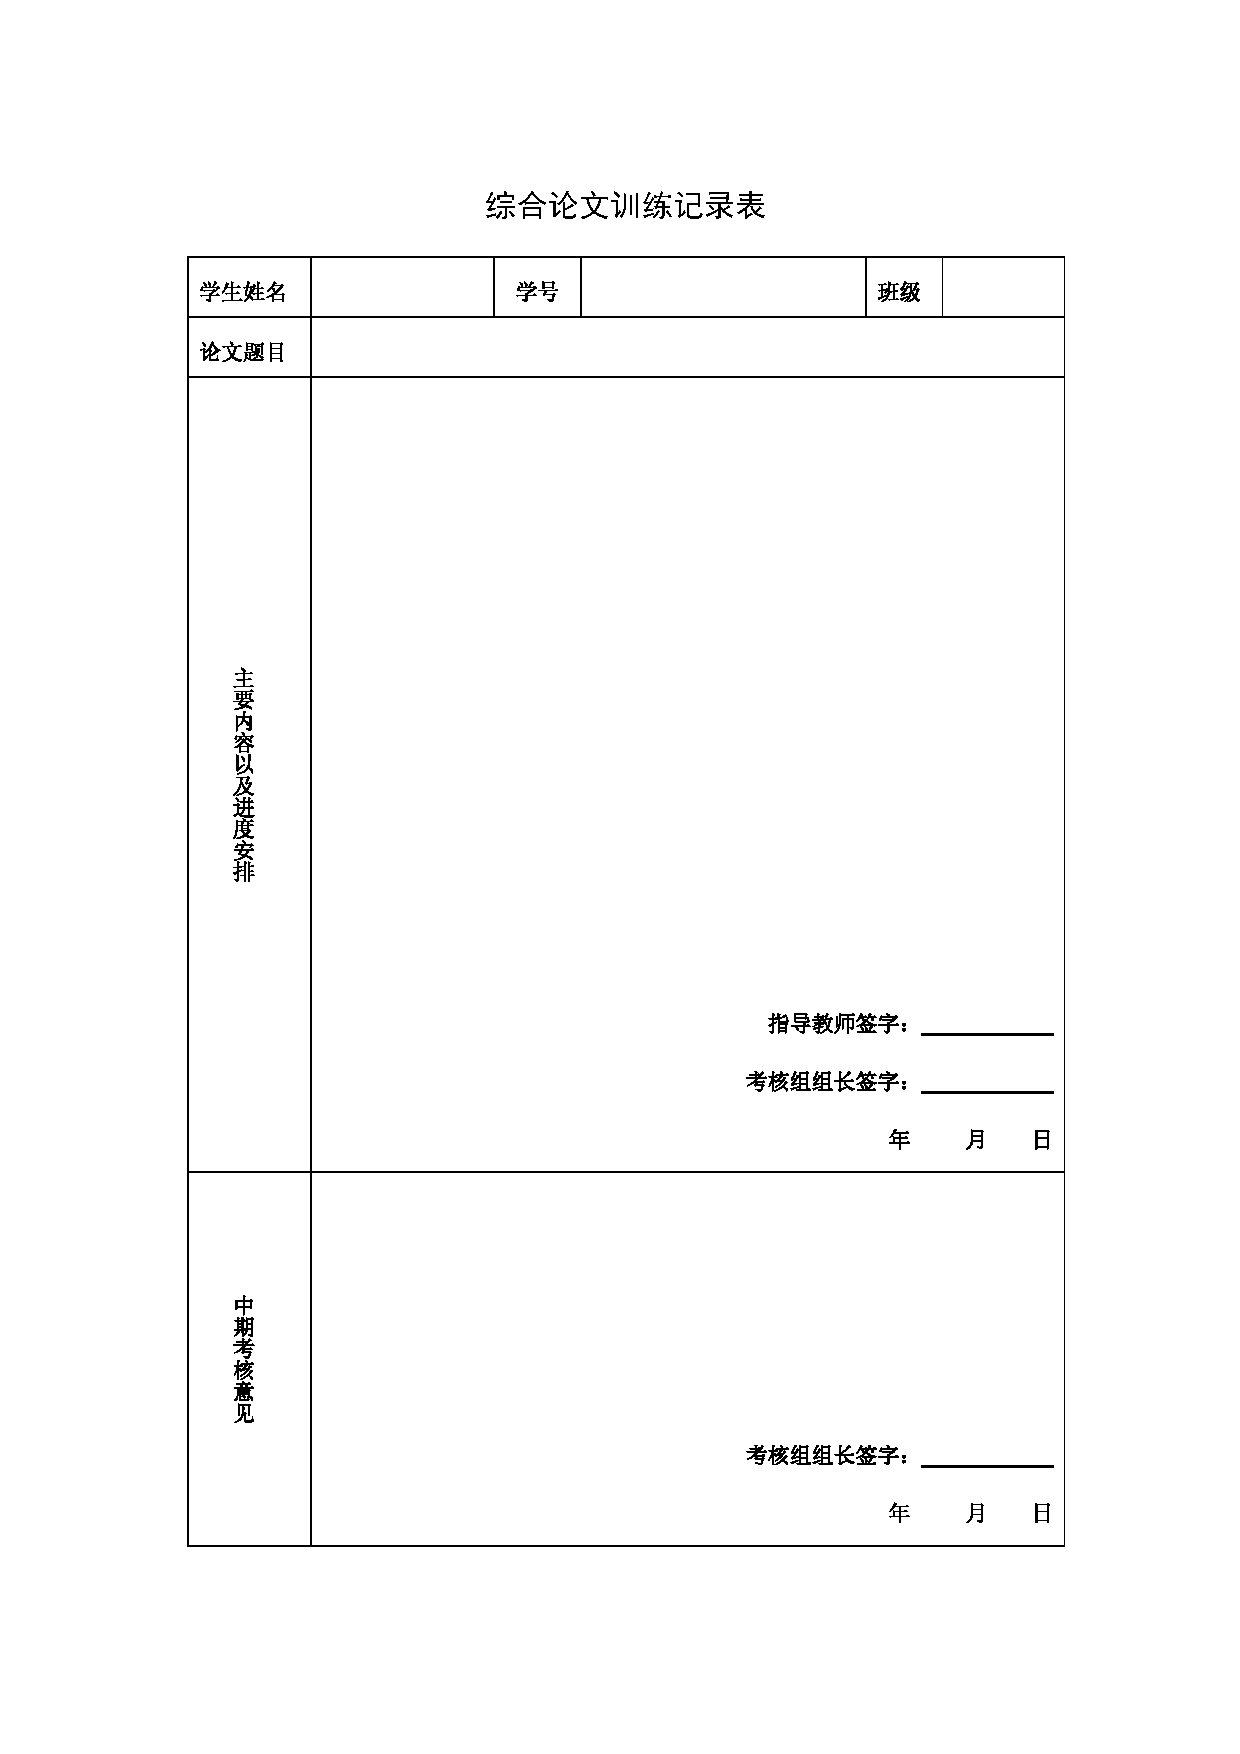
\includepdf[pages=-]{scan-record.pdf}

\end{document}
